\chapter{Linsengesetze}
\label{v:7}

Der praktische Umgang mit Linsen und Linsensystemen soll geübt werden.

%------------------------------------------------
\section{Stichworte}
%------------------------------------------------
Grundbegriffe und Gesetze der geometrischen Optik; Gausssche Linsenformel; Besselsches Verfahren; Bildkonstruktion.
%
%------------------------------------------------
\section{Literatur}
%------------------------------------------------
Gehrtsen, Kapitel 9.1.3 und 9.2.2
%
%------------------------------------------------
\section{Theoretischer Hintergrund}
%------------------------------------------------

Bezeichnet man mit $g$ und $b$ jeweils die Abstände eines abzubildenden Gegenstandes und seines Bildes von der abbildenden Linse, sowie mit $G$ und $B$ die Größe des Gegenstandes bzw. des Bildes, so beschreiben zwei Gleichungen die Abbildung komplett.\\
Die erste Gleichung gibt den Abbildungsmaßstab $\gamma$ an:
\begin{equation} \label{eq:Abbildungsmassstab-Linse}
 \frac{B}{G} = \frac{b}{g} = \gamma\; .
\end{equation}
Die zweite Gleichung, die sogenannte Gausssche Linsenformel, setzt Gegenstands- und Bildweiten in Verbindung mit der Brennweite $f$ der Linse:
\begin{equation} \label{eq:Linsenformel}
 \frac{1}{g} + \frac{1}{b} = \frac{1}{f}\; .
\end{equation}

\noindent
Zur Lösung dieses Gleichungssystems gibt es ein bewährtes, physikalisch interpretierbares graphisches Verfahren. Diese Bildkonstruktion benutzt zwei der drei Strahlen Parallelstrahl, Mittelpunktstrahl und Brennpunktsstrahl.\\

\noindent
Im folgenden wird angenommen, dass das Medium vor und hinter der Linse dasselbe ist. Warum ist das wichtig?

\subsection{Bildkonstruktion}

\textbf{Dünne Linsen}\\
Bei dünnen Linsen führt man die Bildkonstruktion mit zwei Strahlen durch:\\
Ein vom Gegenstand kommender Strahl parallel zur optischen Achse des Aufbaus, welcher in der Mittelebene der Linse H so gebrochen wird, dass er durch den bildseitigen Brennpunkt $f_b$ der Linse geht.\\
Ein vom Gegenstand kommender Strahl, der durch den gegenstandsseitigen Brennpunkt $f_g$ geht, wird in H so gebrochen, dass er parallel zur optischen Achse weiterläuft. Die bild- und gegenstandsseitigen Brennweiten sind gleich.\\
Darüber hinaus existiert ein Mittelpunktstrahl, der Gegenstand und Bild durch den Linsenmittelpunkt geradlinig verbindet.\\
\begin{figure}[h]
	\centering
		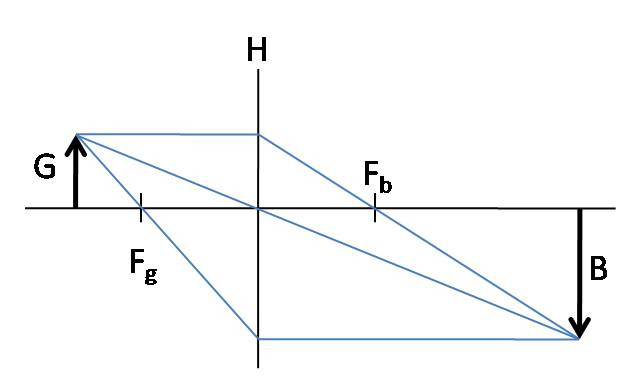
\includegraphics[width=0.5\textwidth]{Versuch_7-8/Abbildungen/duenne_linse.jpg}
	\label{fig:duenne_linse}
\end{figure}


\noindent
\textbf{Dicke Linsen und Linsensysteme}\\
Anders als bei dünnen Linsen gibt es hier keine Mittelebene mit den oben erwähnten Eigenschaften. Es existieren jedoch zwei sogenannte Hauptebenen $H_g$ und $H_b$ mit folgenden Eigenschaften.\\
Ein vom Gegenstand kommender, achsenparalleler Strahl wird in $H_b$ so gebrochen, dass er durch den bildseitigen (System-)Brennpunkt $F_b$ geht.\\
Ein vom Gegenstand durch den gegenstandsseitigen Brennpunkt $F_g$ verlaufender Strahl wird in $H_g$ so gebrochen, dass er achsenparallel weiterläuft.\\
$H_g$ und $H_b$ sind Hilfsmittel zur einfachen Bildkonstruktion, sie müssen nicht mit den Linsenebenen übereinstimmen. Sie können im Extremfall ausserhalb des Linsensystems liegen oder sogar vertauscht sein. 
\begin{figure}[h]
	\centering
		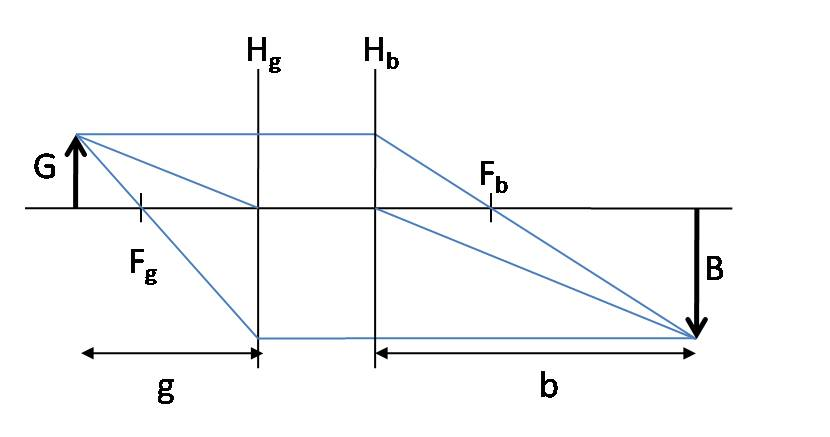
\includegraphics[width=0.5\textwidth]{Versuch_7-8/Abbildungen/dicke_linse.jpg}
	\label{fig:dicke_linse}
\end{figure}

Der Abstand zwischen Brennpunkt und zugehöriger Hauptebene $\left[F_i,\,H_i\right]$ ist auf beiden Seiten des Systems gleich und definiert die Brennweite des Systems:
\[
\left[F_g,\,H_g\right]\,=\,\left[F_b,\,H_b\right]\,=\, f\; .
\]

\noindent
Ein Anleitung zur zeichnerischen Bestimmung der System-Brennpunkte $F_g$, $F_b$ und Hauptebenen $H_g$, $H_b$ findet sich im Anhang.

\subsection{Das Besselsche Verfahren}

Auf einer optischen Bank sind im Abstand $a$ ein Dia (Gegenstand) und eine Mattscheibe (Bild) aufgebaut. Das Dia wird durch eine innerhalb von $a$ verschiebbare Linse auf die Mattscheibe abgebildet. Es ergeben sich zwei Linsenstellungen I und II mit dem Abstand $e$, bei denen ein reelles, scharfes Bild entsteht.\\
\begin{figure}[h]
	\centering
		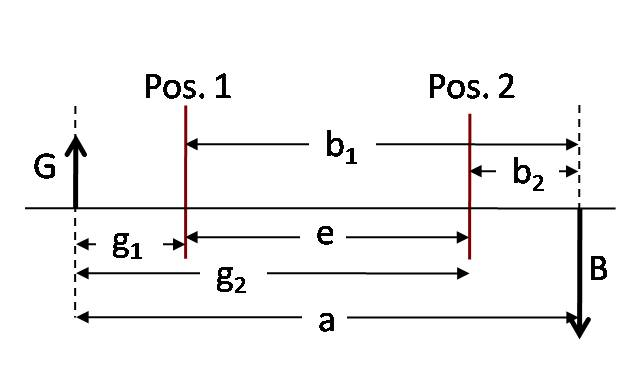
\includegraphics[width=0.5\linewidth]{Versuch_7-8/Abbildungen/bessel_neu.jpg}
	\label{fig:bessel}
\end{figure}

\noindent
Mit der Linsenformel lässt sich die Formel ableiten
\begin{equation}
 4f = \frac{a^2 - e^2}{a}\; ,
\end{equation}
mit der die Brennweite $f$ der Linse oder eines Linsensystems bestimmt werden kann, falls $a \geq 4f$ ist.\\
Der Vorteil des Bessel Verfahrens gegenüber der einfachen Bestimmung der Brennweite einer Linse aufgrund der Linsenformel \ref{eq:Linsenformel} besteht darin, dass für dicke Linsen die Lage der Hauptebenen der Linse nicht bekannt sein müssen. Diese können mit dem etwas aufwendigeren Verfahren nach Abbe jedoch auch bestimmt werden.

\subsection{Anwendung: Menschliches Auge und Sehfehler}

(aus: Winkler/Hintermann: Physik - Repetitorium der Physik, Teil II, Diesterweg, 1978)\\

\noindent
Das menschliche Auge ist im wesentlichen ein System aus zwei Linsen. Die erste Linse besteht aus der Hornhaut und die zweite aus der verformbaren Kristall-Linse. Durch die kombinierte Wirkung dieser beiden Linsen wird das Bild des Gegenstandes, den wir betrachten, auf die hintere Wand des Augapfels geworfen. Diese Wand ist von lichtempfindlichen Nerven bedeckt. Sie wird die \textit{Netzhaut} oder \textit{Retina} genannt. Die Muskeln, welche die Linse tragen, können sie nach Belieben krümmen. Dadurch wird es möglich, dass das Auge Gegenstände in unterschiedlicher Entfernung scharf sehen kann. Es gibt jedoch im menschlichen Auge keine Muskeln, mit denen die Linsenkrümmung verringert werden kann. Wenn das normalsichtige Auge völlig entspannt ist, liegt sein Fernpunkt im Unendlichen, d.h. dass von allen weit entfernten Gegenständen auf der Netzhaut ein scharfes Bild entsteht. Zur Betrachtung von nahen Gegenständen muss durch die Augenmuskeln die Augenlinse stärker gekrümmt werden, damit die Brennweite verkürzt 
wird.
\begin{figure}[h]
	\centering
		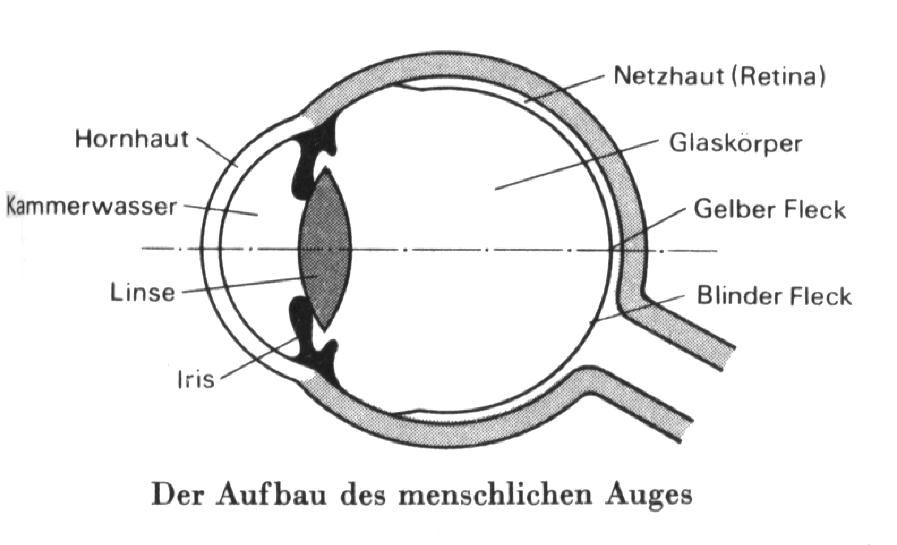
\includegraphics[width=0.5\textwidth]{Versuch_7-8/Abbildungen/auge.jpg}
	\label{fig:auge}
\end{figure}

\noindent
Beim kurzsichtigen Auge ist meistens die Distanz Linse - Netzhaut zu groß, seltener ist die Linse zu stark gekrümmt. Da das menschliche Auge keine Muskeln zur Verringerung der Linsenwölbung des entspannten Zustandes besitzt, besteht in diesem Fall keine Möglichkeit zur Akkomodation. Beim weitsichtigen Auge liegen die Verhältnisse umgekehrt. Im entspannten Zustand können selbst ferne Gegenstände nicht scharf gesehen werden. Die Linse des weitsichtigen Auges steht deshalb, selbst beim Blick in die Ferne, stets unter einem Druck der Augenmuskeln, was zu rascher Ermüdung führt.\\

\noindent
Durch die entsprechenden Linsen können die Sehfehler korrigiert werden:
\begin{figure}[h]
	\centering
		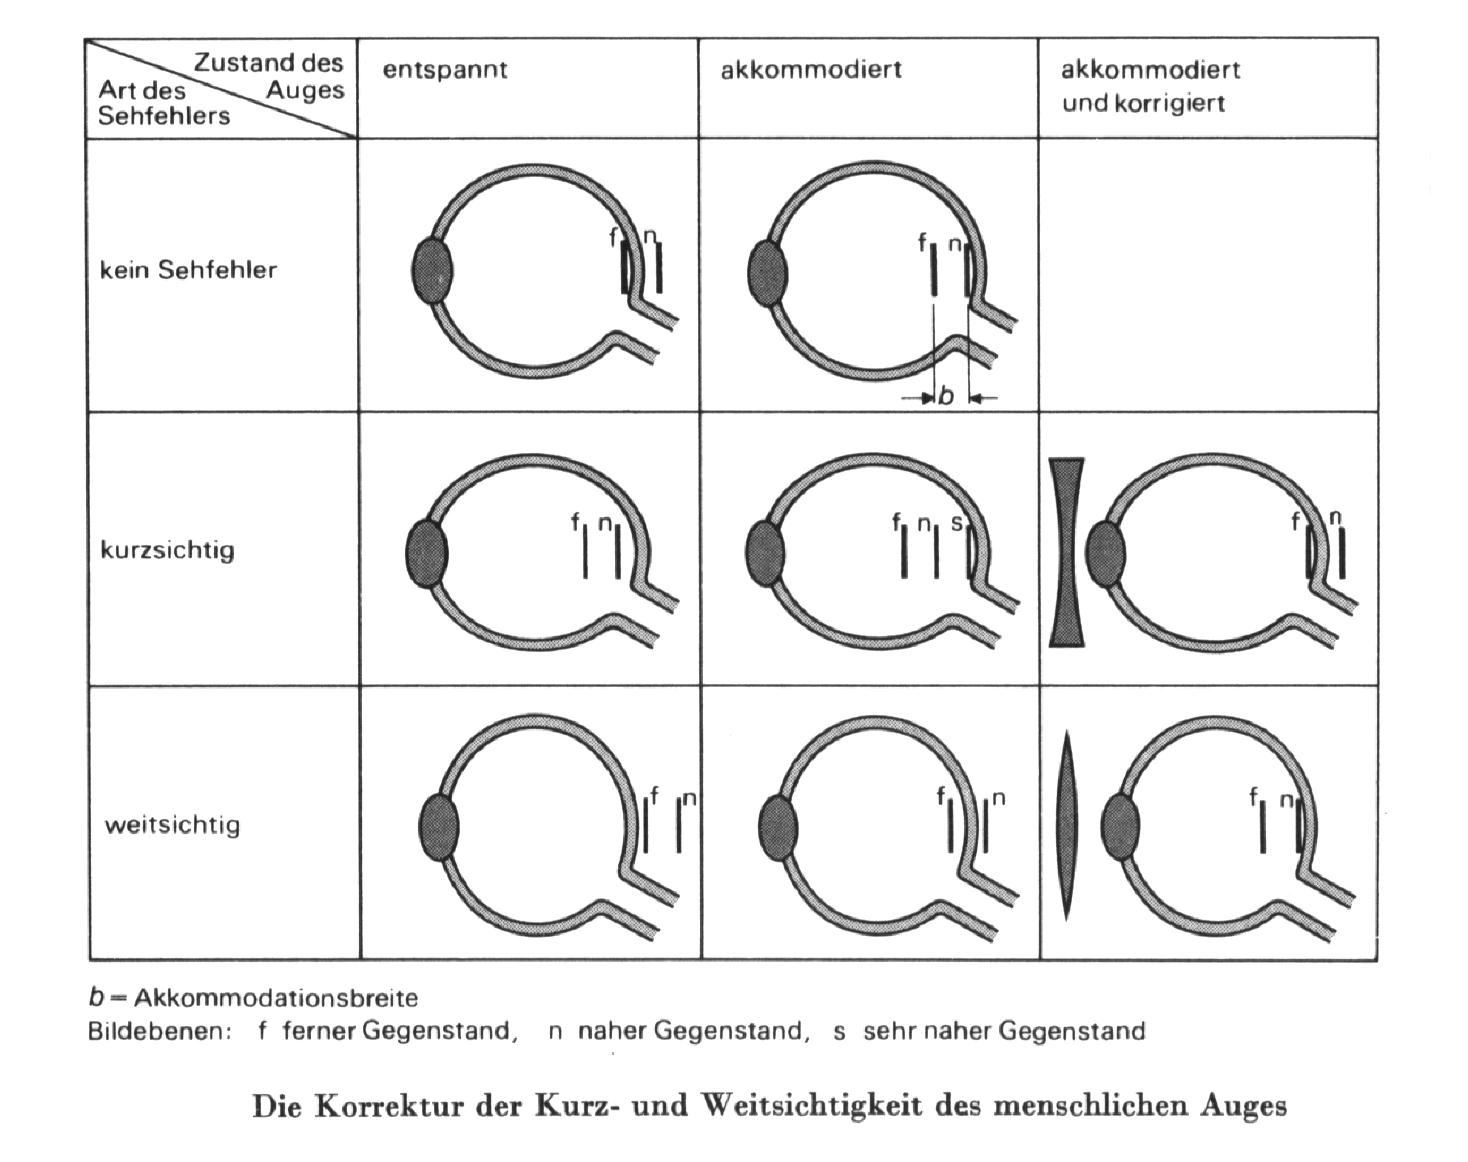
\includegraphics[width=\textwidth]{Versuch_7-8/Abbildungen/Sehfehler.jpg}
	\label{fig:Sehfehler}
\end{figure}

%------------------------------------------------
\section{Fragen zur Vorbereitung}
%------------------------------------------------

\begin{enumerate} 
%\item Was soll heute im Praktikum gemessen werden? Warum?
%
 \item Welche Linsentypen unterscheidet man?
%
\item Wie kann die Vergrößerung einer Linse aus Bildgröße $B$ und Gegenstandsgröße $G$ berechnet werden?
%
\item Was ist ein virtuelles/reales Bild?
%
\item Wie lautet die Linsenformel (mit Strahlengang)?
%
\item Wie berechnet man die Brennweite einer Linsenkombination?
%
\item Was ist eine Dioptrie?
%
\item Wozu dient das Besselverfahren?
%
\item Wann existieren a) eine Linsenstellung, b) zwei Linsenstellungen und c) keine Linsenstellung, bei denen ein Gegenstand scharf abgebildet wird? (Die Frage bezieht sich auf das Besselverfahren)
\end{enumerate} 

%------------------------------------------------
\section{Durchführung} 
%------------------------------------------------

 Fur jedes $a$ ist $e$ jeweils fünfmal zu messen.

\begin{enumerate}
 %
 \item Stellen Sie für die Sammellinse den Gegenstandsabstand ein auf jeweils $a$ = 45, 50, 60, 70, 80~cm.
 %
 \item Für die Kombination aus Sammel- und Zerstreuungslinse messen Sie nur für $a$ = 100~cm.
\end{enumerate}

%------------------------------------------------
\section{Auswertung} 
%------------------------------------------------
Bemerkung: Die benötigten Formeln für Mittelwert, Standartabweichung des Mittelwerts, Fehlerfortpflanzung, etc. sind der Anleitung zur 'Fehlerrechnung im Nebenfachpraktikum' zu entnehmen.

\begin{enumerate}
%
\item Berechnen sie den Mittelwert $\overline{e}$ von $e$ für jede Basislängen $a$ und bestimmen sie den dazugehörigen Fehler über die \textbf{Standardabweichung des Mittelwerts}.
%
\item Errechnen sie die Brennweiten $f_s$ der Sammellinse für die verschiedenen Einstellungen der Basislänge $a$ und die Brennweite $f_k$ der Linsenkombination über 
\begin{equation*}
f_{s,k} = \frac{a^2-e^2}{4 a}
\end{equation*}
Verwenden sie dafür die jeweils berechneten Werte von $\overline{e}$.
%
\item Ermitteln sie die Fehler $\Delta f_{s,k}$ der Brennweiten ($f_s$ und $f_k$). Nutzen sie dafür die Fehlerforpflanzung und bedenken sie, dass sowohl $\overline{e}$ als auch $a$ fehlerbehaftet Größen sind. Rechnen sie die für die Fehlerforpflanzung nötigen Ableitungen explizit aus! Nehmen sie als Fehler für a $\Delta a = 0,5$ mm an. Warum ist diese Annahme sinnvoll?
Tip: Fehler für Sammellinse und Kombination:
\begin{equation*}\Delta f_{s,k}=\sqrt{\left(\frac{\partial f_{s,k}}{\partial a} ~ \Delta a\right)^2 + \left(\frac{\partial f_{s,k}}{\partial e} ~ \Delta e\right)^2}
\end{equation*}
%
\item Berechnen sie aus den Brennweiten der Sammellinse und den dazugehörigen Fehlern das \textbf{gewichtete} Mittel $\overline{f}_s$ und den entsprechenden Fehler $\Delta \overline{f}_s$.
%
\item Bestimmen sie aus $\overline{f}_s$ und $f_k$ die Brennweite der Zerstreuungslinse $f_z$ und dessen Fehler $\Delta f_z$ über die Fehlerfortpflanzung, nutzen sie dazu:
\begin{equation*}
f_Z = \frac{1}{\frac{1}{f_k} - \frac{1}{f_s}}
\end{equation*}
Rechnen sie auch hier die für die Fehlerforpflanzung nötigen Ableitungen expizit aus.
\textbf{Achtung}: hier ist nicht nach $\Delta \frac{1}{f_z}$ gefragt!
%
\item Diskutieren sie entscheidende Fehlerquellen in diesem Versuch.
%
\end{enumerate}